\section{Kalman Filter}
\label{kalman_filters}

\begin{figure}[!htb]
\begin{center}
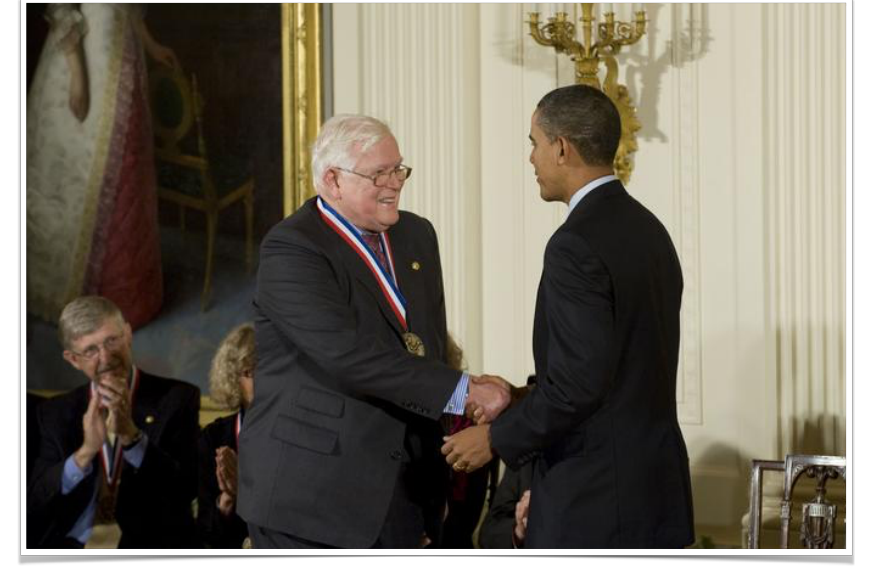
\includegraphics[scale=0.280]{img/kalman_filter/rudolf_e_kalman.jpeg}
\end{center}
\caption{Rudolf E. Kálmán receiving the National Medal of Science.}
\label{rudolf_e_kalman}
\end{figure}


In this section, we'll learn about one of the most famous algorithms in all of engineering; namely the Kalman filter. In today's world of
advanced machine learning, the Kalman filter remains
an important tool to fuse measurements from several sensors to estimate in real-time the state of a robotic system such
as a self-driving car. Concretely, in this section, we will introduce its basic linear formulation and also show  why the Kalman filter is the best linear unbiased
estimator. 

\section{Introduction}
\label{kalman_filter_introduction}

The Kalman filter algorithm was
published in 1960 by Rudolf E. Kalman, a Hungarian born professor
and engineer who was working at the Research Institute
for Advanced Studies in Baltimore Maryland. Years later in 2009, American President Barack
Obama awarded Kalman the prestigious National Medal
of Science for his work on the Kalman filter and other contributions to the field
of control engineering.

After its publication in 1960, the Kalman filter was adopted by NASA for use in
the Apollo guidance computer. 

\begin{figure}[!htb]
\begin{center}
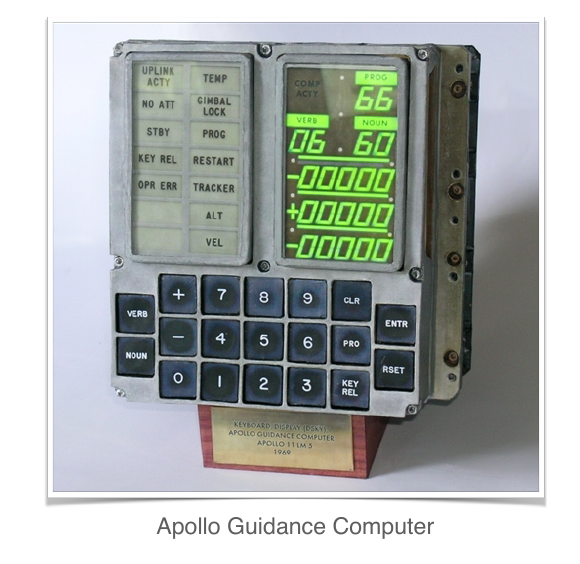
\includegraphics[scale=0.280]{img/kalman_filter/apollo_guidance_computer.jpeg}
\end{center}
\caption{The Apollo guidance computer used Kalman filtering.}
\label{apollo_guidance_computer}
\end{figure}

It was this ground-breaking innovation
that played a pivotal role in successfully getting
the Apollo spacecraft to the moon, and to our first steps on another world. The filter helped guide the Apollo spacecraft accurately
through its circumlunar orbit. 

The engineers at
NASA's Ames Research Center, adopted Kalman's linear theory and
extended it to nonlinear models. We will discuss this specific extension
in a later section. But first, let's talk about
the basic linear Kalman filter. 

\section{Linear Kalman Filter}


The Kalman filter is very similar to the linear recursive least squares
filter we discussed earlier. While recursive least squares updates
the estimate of a static parameter, but Kalman filter is able to update
and estimate of an evolving state. Thus, Kalman filtering is an iterative process that uses a set of equations and consecutive data inputs to quickly estimate the 
true value; e.g. position, velocity etc., of the object being measured when the measured values contain unpredicted or 
random error, uncertainty or variation.


The goal of the Kalman filter is to take a probabilistic estimate
of this state and update it in real time using
two steps; prediction and correction. 


To make these ideas more concrete, let's consider a problem of estimating
the 1D position of the vehicle. 

\begin{figure}[!htb]
\begin{center}
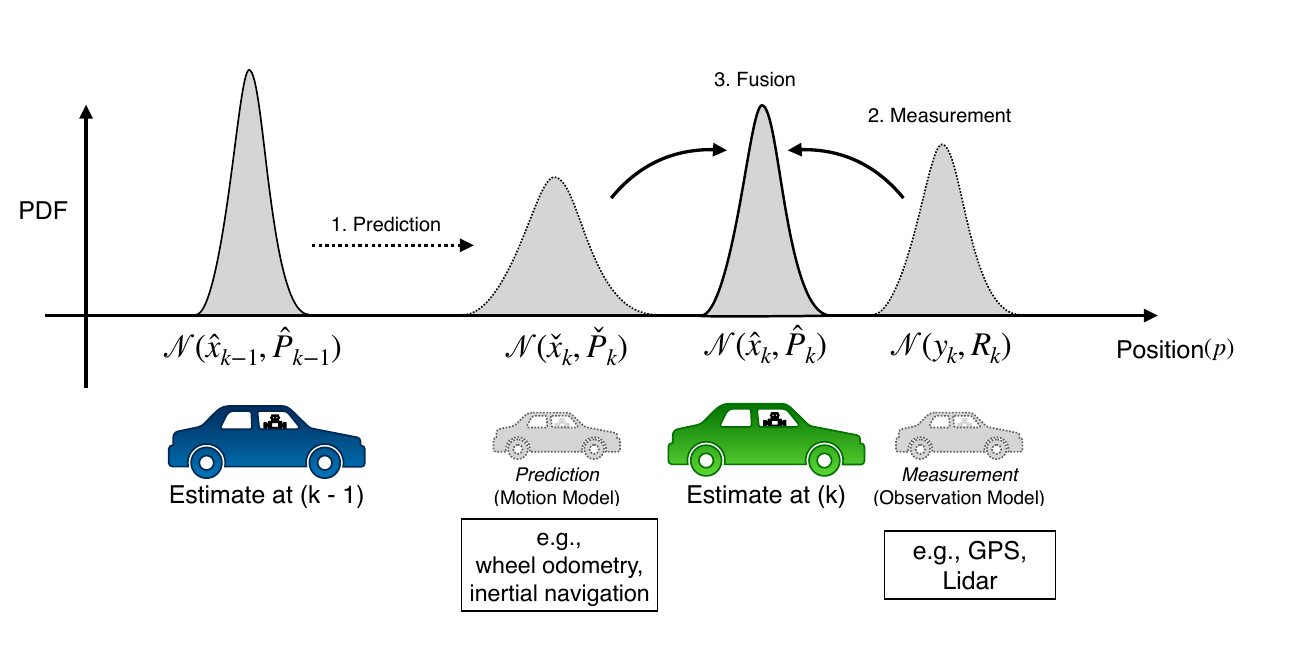
\includegraphics[scale=0.280]{img/kalman_filter/kalman_1.jpeg}
\end{center}
\caption{The Apollo guidance computer used Kalman filtering.}
\label{kalman_1}
\end{figure}

Starting from an initial probabilistic
estimate at time $k-1$, our goal is to use a \textbf{motion model}
which could be derived from wheel odometry or inertial sensor
measurements to predict our new state. Then, we'll use the observation model
derived from GPS for example, to correct that prediction
of vehicle position at time $k$. 

Each of these components, the initial estimate, the predicted state, and
the final corrected state are all random variables that we will specify
by their means and covariances. In this way, we can think of the Kalman filter as a technique to fuse information from
different sensors to produce a final estimate of some unknown state, taking into account, uncertainty
in motion and in our measurements. For the Kalman filter algorithm, we had been able to write
the motion model in the following way; the estimate at time step k is a linear combination of the estimate
at time step $k-1$, a control input and some zero-mean noise. 


The input is an external signal that affects the evolution of our system state. In the context of self-driving vehicles, this may be a wheel torque applied to speed up and change lanes, for example. Next, we will also need to define
a linear measurement model. Finally, we'll need a measurement
noise as before and a process noise that
governs how certain we are that our linear dynamical system
is actually correct, or equivalently, how uncertain we are about the effects
of our control inputs. 

\begin{eqnarray}
\mathbf{x}_k = \mathbf{F}_{k-1}\mathbf{x}_{k-1} + \mathbf{G}_{k-1}\mathbf{u}_{k-1} + \mathbf{w}_{k-1} \\
\mathbf{y}_k = \mathbf{H}_k \mathbf{x}_k + \mathbf{v}_k
\end{eqnarray}

where

\begin{equation}
\mathbf{v}_k \sim N(0, \mathbf{R}_k), ~~ \mathbf{w}_k \sim N(0, \mathbf{Q}_k) 
\end{equation}

Once we have our system in hand, we can use an approach
very similar to that we discussed in the recursive
least squares. Except this time, we'll
do it in two steps. 

\begin{itemize}
\item First, we use the process model to predict how our states, remember, that we're now typically talking
about evolving states and non-state parameters evolved since the last time step, and will propagate our uncertainty. 
\item Second, we'll use our measurement to correct that prediction based on our measurement residual
or innovation and our optimal gain. 
\end{itemize}

Finally, we'll use the gain to also propagate the state covariance from our prediction
to our corrected estimate. This is shown in Figure

\begin{figure}[!htb]
\begin{center}
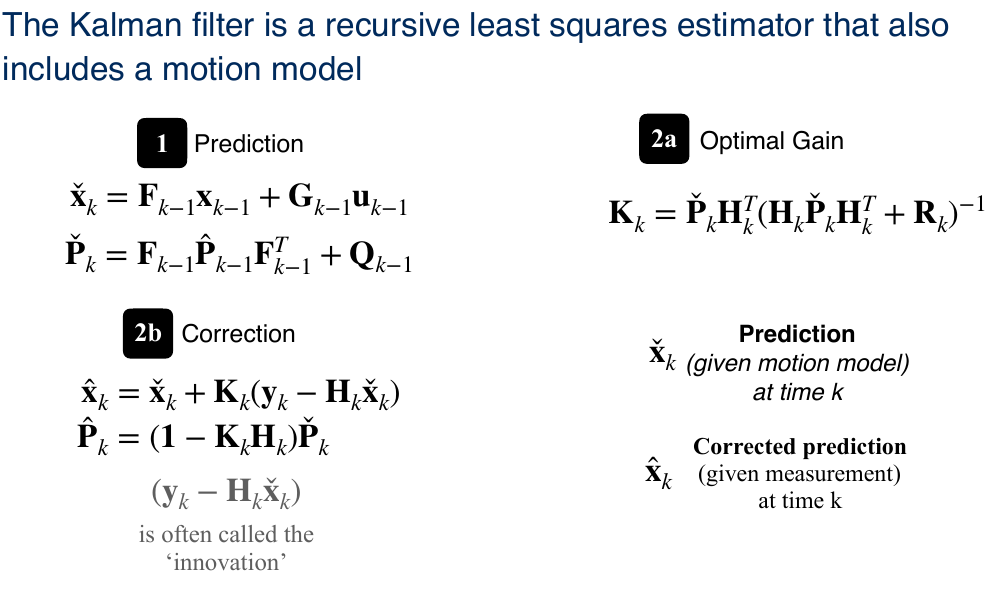
\includegraphics[scale=0.280]{img/kalman_filter/kalman_2.jpeg}
\end{center}
\caption{The linear Kalman filter steps.}
\label{kalman_2}
\end{figure}

In our notation, the hat indicates a corrected prediction
at a particular time step. Whereas a check indicates a prediction before
the measurement is incorporated. If you've worked with the
Kalman filter before, you may also have seen this
written with plus and minus signs for the corrected and
predicted quantities, respectively. 

Let's recap. We start with
a probability density over our states and also maybe parameters
at time step $k-1$, which we represent as
a multivariate Gaussian. We then predict the states
at time step $k$ using our linear prediction model and propagate both the mean
and the uncertainty; the covariance, forward in time. Finally, using our probabilistic
measurement model, we correct our initial
prediction by optimally fusing the information from
our measurement together with the prior prediction through our optimal
gain matrix $\mathbf{K}$. Our end result is an updated probabilistic estimate
for our states at time step $k$. 

\begin{figure}[!htb]
\begin{center}
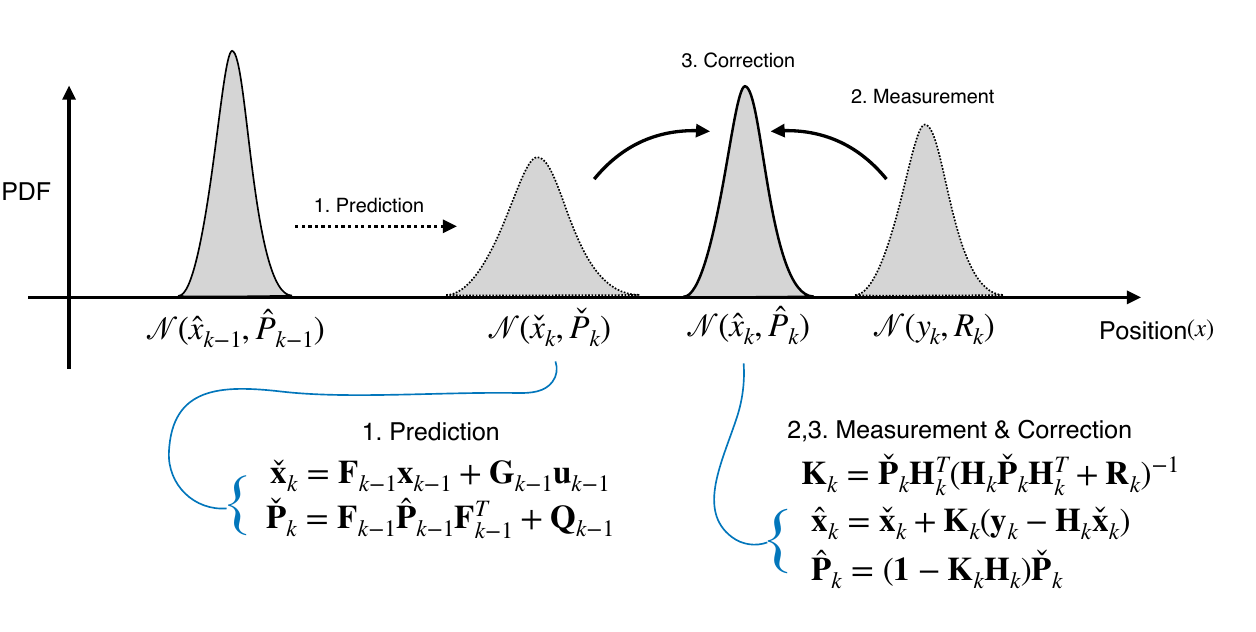
\includegraphics[scale=0.280]{img/kalman_filter/kalman_3.jpeg}
\end{center}
\caption{The linear Kalman filter steps.}
\label{kalman_3}
\end{figure}

\subsection{Example: 1D Vehicle Motion}

The best way to become comfortable with the
Kalman filter is to use it. Let's look at a simple example. Consider again the case of the self-driving vehicle
estimating its own position. Our state vector will include the vehicle position and
its first derivative velocity. Our input will be a scalar acceleration
that could come from a control system that commands our car
to accelerate forward or backwards. For our measurement, we'll assume
that we're able to determine the vehicle position directly using
something like a GPS receiver. Finally, we'll define
our noise variances as follows: Given this initial
estimate and our data, what is our corrected position
estimate after we perform one prediction step and one correction
step using the Kalman filter? Here's, how we can use
these definitions to solve for our corrected position
and velocity estimates. Pay attention to the fact that our final corrected state
covariance is smaller. That is we are more certain about the car's position after we
incorporate the position measurement. This uncertainty reduction occurs because our measurement model
is fairly accurate. That is, the measurement noise
variance is quite small. Try increasing
the measurement variance and observe what happens to
the final state estimate. To summarize, the Kalman filter is
similar to recursively squares, but also adds a motion model that
defines how our state evolves over time. The Kalman filter works
in two stages: First, predicting the next state
using the motion model, and second, correcting
this prediction using a measurement. But how can we be sure
that the Kalman filter is giving us an accurate state estimate? 


\section{Kalman Filter and BLUE}
\label{kalman_filter_blue}

We have introduced the Kalman Filter, let's discuss little bit about what makes
it such an appealing estimation method. 

\subsection{Bias}
\label{kalman_filter_bias}

Let's dive in. First, let's discuss bias. Let's consider our Kalman Filter
from the previous lesson and use it to estimate the position
of our autonomous car. If we have some way of knowing the true
position of the vehicle, for example, an oracle tells us, we can then use this to record a position
error of our filter at each time step $k$. Since we're dealing with random noise,
doing this once is not enough. We will need to repeat this same
process over and over and record our position
error at each time step. Once we've collected these errors, if they
average to zero at a particular time step $k$, then we say the Kalman Filter
estimate is unbiased at this time step.  Graphically, this is what the situation may look like. 

\begin{figure}[!htb]
\begin{center}
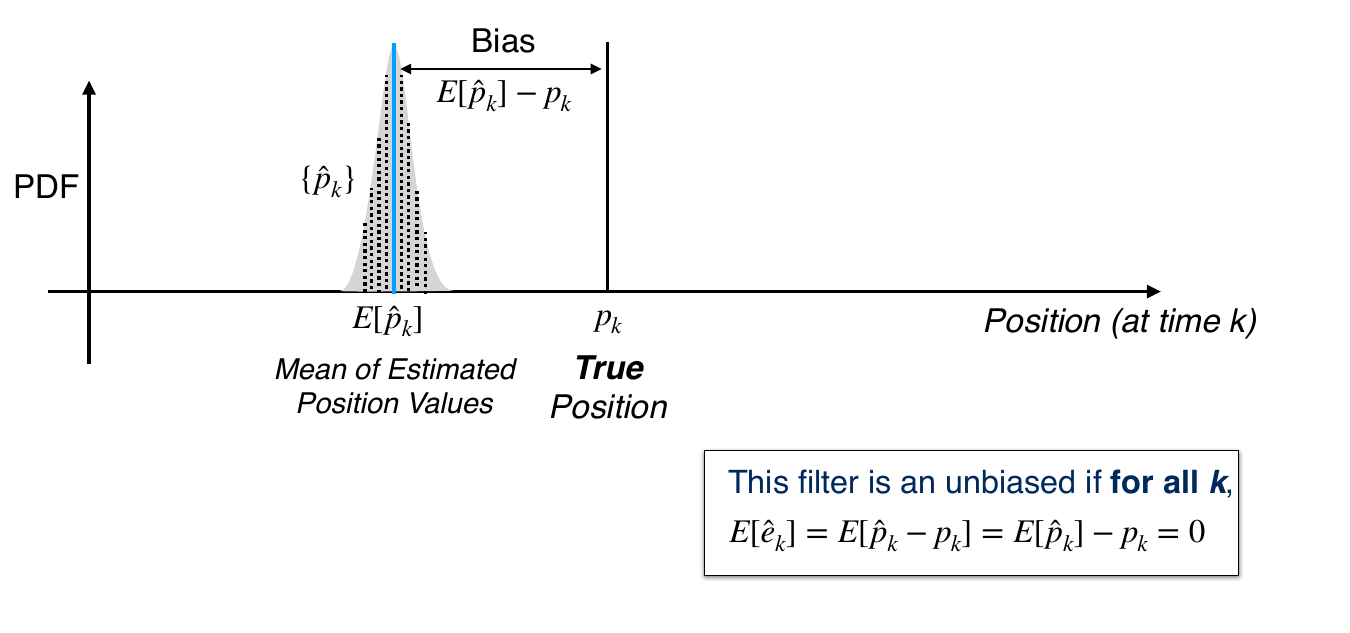
\includegraphics[scale=0.280]{img/kalman_filter/kalman_4.jpeg}
\end{center}
\caption{The linear Kalman filter steps.}
\label{kalman_4}
\end{figure}

Say the particular time step, we know that the true position is the following. We build a histogram of the positions that
our filter reports over multiple trials, and then compute the difference between
the average of these estimates and the true position. If this difference does not approach zero,
then our estimate is biased. However, if this difference does approach
zero as we repeat this experiment many more times, and
if this happens for all time intervals, then we say that our filter is unbiased. Although we could potentially verify
this lack of bias empirically, what we'd really like are some
theoretical guarantees. 

Let's consider the error dynamics of our filter. We define our predicted and corrected state
errors as follows

\begin{eqnarray}
\text{Predicted state error: }~~\check{\mathbf{e}}_k = \check{\mathbf{x}}_k - \mathbf{x}_k\\
\text{Corrected estimate error: }~~\hat{\mathbf{e}}_k = \hat{\mathbf{x}}_k - \mathbf{x}_k
\end{eqnarray}

We can then use the common filter equations to write
the following relations. 

\begin{eqnarray}
\check{\mathbf{e}}_k = \mathbf{F}_{k-1}\check{\mathbf{e}}_{k-1} - \mathbf{w}_k \\
\hat{\mathbf{e}}_k = (\mathbf{I} - \mathbf{K}_k\mathbf{H}_k)\check{\mathbf{e}}_k + \mathbf{K}_k\mathbf{v}_k
\end{eqnarray}

For the Kalman Filter, we can show the expectation value of
these errors is equal to zero exactly. Meaning that we can show

\begin{equation}
E[\check{\mathbf{e}}_k] = \mathbf{0}, ~~ E[\hat{\mathbf{e}}_k] = \mathbf{0}
\end{equation}

For this to be true, we need to ensure that our initial state estimate is unbiased and that our noise is white,
uncorrelated, with zero mean. While this is a great result for linear systems, remember that this doesn't guarantee that
our estimates will be error free for a given trial, only that the expected
value of the error is zero. 

\subsection{Consistency}
\label{kalman_filter_consistency}

Kalman Filters are also what is called consistent. By consistency we mean that for
all time steps $k$, the filter covariants $P_k$ matches the expected
value of the square of our error. 

\begin{figure}[!htb]
\begin{center}
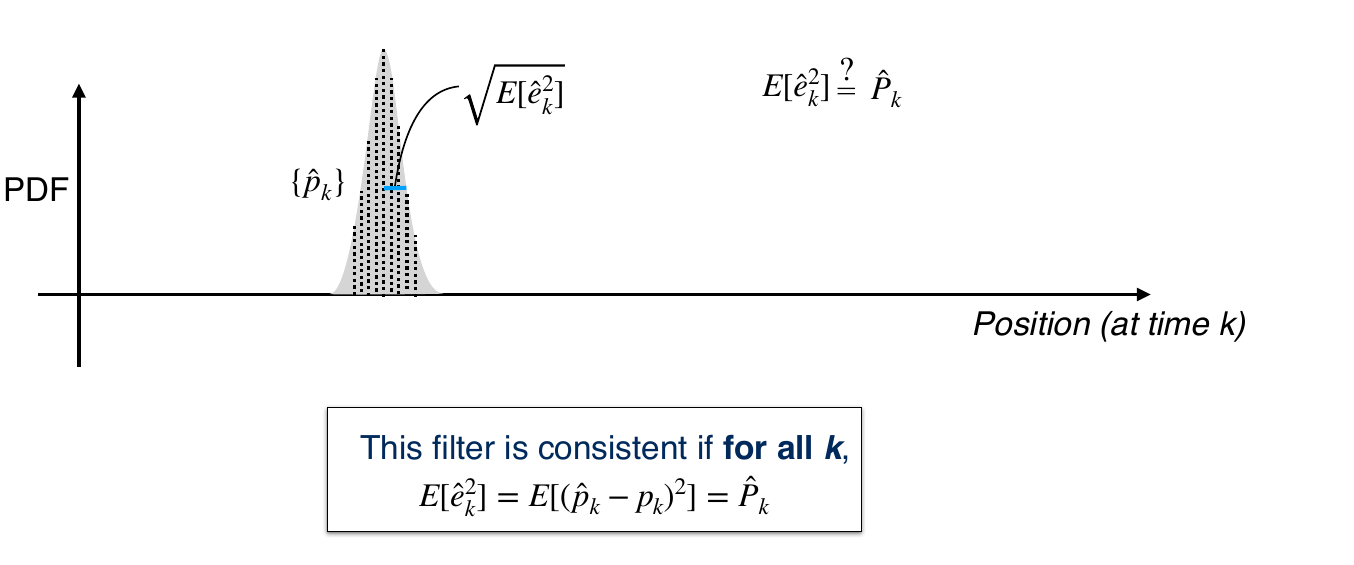
\includegraphics[scale=0.280]{img/kalman_filter/kalman_5.jpeg}
\end{center}
\caption{The linear Kalman filter steps.}
\label{kalman_5}
\end{figure}

For scalar parameters,
this means that the empirical variance of our estimate should match
the variance reported by the filter. Practically, this means that our
filter is neither overconfident, nor underconfident in
the estimate it has produced. 

\subsubsection{Overconfident filter}

A filter that is overconfident,
and hence inconsistent, will report a covariance
that is optimistic. That is, the filter will essentially place
too much emphasis on its own estimate and will be less sensitive to
future measurement updates, which may provide critical information. It's easy to see how an overconfident
filter might have a negative or dangerous effect on the performance
of self-driving car. 


So long as our initial
estimate is consistent, and we have white zero mean noise,
then all estimates will be consistent. Putting everything together,
we've shown that given white uncorrelated zero mean noise, the Kalman
Filter is unbiased and consistent. Because of these two facts, we say that the Kalman Filter is the BLUE,
the Best Linear Unbiased Estimator. It produces unbiased estimates with
the minimum possible variance. 

To summarize, in this section we've defined the terms bias and consistency, and
showed that the Kalman Filter is unbiased, consistent, and the Best Linear
Unbiased Estimator, or BLUE. Remember that best here refers to
the fact that the Kalman Filter minimizes the state variance. Although this is a fantastic result,
most real systems are not linear. For self-driving cars, we'll
generally need to estimate non-linear quantities like vehicle poses,
position, and orientation in 2D and 3D. To do this, we'll need to extend the linear
Kalman Filter into the non-linear domain. 


\subsection{Kalaman Gain}
The Kalman gain $K$is used to determine how much of the new measurements to use in order to update the new estimate.
In the caluclation of the Kalman gain two quantities participate:

\begin{itemize}
\item Error in estimate
\item Error in data measurement
\end{itemize}

Thus $K$ is given by

\begin{equation}
K = \frac{E_{est}}{E_{est} + E_{meas}}
\label{kalman_gain}
\end{equation} 

From equation \ref{kalman_gain} it follows that

\begin{equation}
0 \leq K \leq 1
\label{kalman_gain_condition}
\end{equation} 

The Kalman gain is the used used to update the current estimate $\hat{x}_t$:

\begin{equation}
\hat{x}_t = \hat{x}_{t-1} + K (z - \hat{x}_{t-1})
\label{new_estimate}
\end{equation} 


When $K \approx 1$ or is equal to one, the measurements we are getting a very accurate however the estimates are unstable. On the other hand when $K$ is small, 
the measurements we are getting a inaccurate but the estimates are stable since the error is small.
The error $E_{\hat{x}}$ in the estimate is given by 

\begin{equation}
E_{\hat{x}_t} = (1-K)E_{\hat{x}_{t-1}}
\label{estimate_error}
\end{equation}

\subsection{Calculations of Kalaman Filter}
The Kalman filter iterates over the following three calculations:

\begin{itemize}
\item Calculate $K$ using equation \ref{kalman_gain}
\item Calculate the new estimate using equation \ref{new_estimate} 
\item Caluclate the error in the estimate using equation \ref{estimate_error}
\end{itemize}


\subsubsection{Example: Temperature Estimate}



\section{Multidimensional Case}

Let's now turn attention to the multidimensional case. Let's introduce some notation. Let $X_0$ and $P_0$ be the initial state.
The matrix $X_0$ contains the initial state of the system. The matrix $P_0$ is the initial process covariance matrix. The process
covariance matrix represents the error in the estimate.


\begin{framed}
\theoremstyle{remark}
\begin{remark}{\textbf{Covariance Matrix}}

A covariance matrix, also known as auto-covariance matrix, dispersion matrix, variance matrix, or variance–covariance matrix, 
is a matrix whose element in the $i, j$ position is the covariance between the $i-th$ and $j-th$ elements of a random vector. 
A random vector is a random variable with multiple dimensions. 
Each element of the vector is a scalar random variable. 
Each element has either a finite number of observed empirical values or a finite or infinite number of potential values. 
The potential values are specified by a theoretical joint probability distribution. 
\end{remark}
\end{framed}



\begin{framed}
\theoremstyle{remark}
\begin{remark}{\textbf{Nonlinear Systems}}

The definition above holds for nonlinear systems as well, and the results discussed here have extensions to the nonlinear case.
\end{remark}
\end{framed}


One of the principal uses of observers in practice is to estimate the state of a
system in the presence of noisy measurements. We have not yet treated noise in our
analysis, and a full treatment of stochastic dynamical systems is beyond the scope
of this text. In this section, we present a brief introduction to the use of stochastic
systems analysis for constructing observers. We work primarily in discrete time to
avoid some of the complications associated with continuous-time random processes
and to keep the mathematical prerequisites to a minimum. This section assumes
basic knowledge of random variables and stochastic processes; see Kumar and
Varaiya [KV86] or Åström [Åst06] for the required material.




Consider again the LTI state-space model

\begin{equation}
\frac{dx}{dt} = Ax + Bu +v  ~~ y = Cx + Du +w 
\end{equation}
the model is augmented with additional terms representing the error or disturbance. Concretely,
$v$ is the process disturbance and $w$ is measurements noise. Both are assumed to be normally distibuted with zero mean;

\begin{eqnarray}
E[v] = 0, ~~ E[vv^T] = R_v, ~~ E[w] = 0, ~~ E[ww^T] = R_w 
\label{noise_proccess_1} 
\end{eqnarray}



\begin{framed}
\theoremstyle{remark}
\begin{remark}{\textbf{Normally distributed random variable}}

A one dimensional random variable $X$ is said to follow the normal distribution
\end{remark}
\end{framed}


\begin{framed}
\theoremstyle{remark}
\begin{remark}{\textbf{Nonlinear Systems}}

The definition above holds for nonlinear systems as well, and the results discussed here have extensions to the nonlinear case.
\end{remark}
\end{framed}

$R_v$ and $R_w$ are the covariance matrices for the process disturbance $v$ and the measurement noise $w$ respectively. Furthermore, we assume that the variables $v, w$ are not correlated i.e 

\begin{eqnarray}
E[vw^T] = 0
\label{noise_proccess_2} 
\end{eqnarray}


\begin{framed}
\theoremstyle{remark}
\begin{remark}{\textbf{Corralated random variables}}

Two random variables $X$ and $Y$ are said to be linearly correlated 
\end{remark}
\end{framed}

The initial condition is also modeled as a Gaussian random variable

\begin{eqnarray}
E[x(0)] = x_0, ~~ E[x(0)x^{T}(0)] = P_0
\label{noise_proccess_3} 
\end{eqnarray}

Implementation of the state-space model in a computer requires discretization. Thus the system can be written as discrete-time linear system with dynamics governed by

\begin{equation}
x_{t+1} = Ax_t + Bu_t + Fv_t,  ~~ y_t = Cx_t + w_t 
\end{equation}

Given the measurements $\{y(\tau), 0 \leq \tau \leq t \}$, we would like to find an estimate $\hat{x}_t$ that minimizes the mean square error:

\begin{equation}
E[(x_t - \hat{x}_t)(x_t - \hat{x}_t)^T] 
\end{equation}

\begin{framed}
\theoremstyle{theorem}
\begin{theorem}{\textbf{Kalman 1961}}


Consider the random process $x_t$ with dynamics described by  

\begin{equation}
x_{t+1} = Ax_t + Bu_t + Fv_t,  ~~ y_t = Cx_t + w_t \nonumber
\end{equation} 

and noise processes and initial conditions described by \ref{noise_proccess_1},  \ref{noise_proccess_2} and 
\ref{noise_proccess_3}. The observer gain $L$ that minimizes the mean square error is given by  

\begin{equation}
L_t = AP_tC^T(R_w + CP_tC^T)^{-1}  \nonumber
\end{equation}

where

\begin{equation}
P_{t+1} =  (A − LC)P_t(A − LC)^T + R_v LR_w L^T, ~~ P_0 = E[x_0x^{T}_0\}
\end{equation}

\end{theorem}
\end{framed}

A proof of this result can be found in \cite{Astrom}. We, note, however the following points:

\begin{itemize}
\item the Kalman filter has the form of a recursive filter: given mean square error $P_t$ at time $t$, we can compute how the estimate and error change. Thus we do not need to keep track of old values of the output.
\item Furthermore, the Kalman filter gives the estimate $\hat{x}_t$ and the error covariance $P_t$, so we can see how reliable the estimate is. 
It can also be shown that the Kalman filter extracts the maximum possible information about output data. 
If we form the residual between the measured output and the estimated output,
\end{itemize}

\begin{equation}
e_t = y_t - C\hat{x}_t
\end{equation}
we can show that for the Kalman filter the error covariance matrix $R_e$ is

\begin{equation}
R_e(i,j) = E(e_{j}e_{k}^{T}) = W_t\delta_{jk} 
\end{equation}

In other words, the error is a white noise process, so there is no remaining dynamic information content in the error.




\begin{framed}
\theoremstyle{theorem}
\begin{theorem}{\textbf{Kalman-Bucy 1961}}


The optimal estimator has the form of a linear observer 

\begin{equation}
\frac{d\hat{x}}{dt} = A\hat{x} + Bu + L(y - C\hat{x}),  ~~ \hat{x}(0) = E(x(0)) \nonumber
\end{equation} 

where $L$ is given by

\begin{equation}
L = PC^TR_{w}^{-1}  \nonumber
\end{equation}

where $P$

\begin{equation}
P(t) = E((x(t)-\hat{x}(t))(x(t)-\hat{x}(t))^T)  \nonumber
\end{equation}

\end{theorem}
\end{framed}


All matrices $A, B, C, R_v, R_w, P$ and $L$ can be time varying. The essential condition is that the Riccati equation (8.30) has a unique positive 
solution.

\section{Kalman’s Decomposition of a Linear System}

We have already seen that two fundamental properties
of a linear input/output system are:

\begin{itemize}
\item reachability 
\item observability
\end{itemize}

It turns out that these two properties can be used to classify the dynamics of a system. The key
result is Kalman’s decomposition theorem, which says that a linear system can be
divided into four subsystems:

\begin{itemize}
\item $\Sigma_{ro}$ which is reachable and observable
\item $\Sigma_{r\bar{o}}$ which is reachable but no observable 
\item $\Sigma_{\bar{r}o}$ which is not reachable but is observable
\item $\Sigma_{\bar{r}\bar{o}}$which is neither reachable nor observable
\end{itemize}


Thus, from the input/output point of view, it is only the reachable and observable
dynamics that matter.

\begin{framed}
\theoremstyle{remark}
\begin{remark}{\textbf{Kalman's decomposition for state-space}}

The general case of the Kalman decomposition is more complicated and requires some additional linear algebra; 
see the original paper by Kalman, Ho, and Narendra [KHN63]. The key result is that the state space can still be decomposed
into four parts, but there will be additional coupling so that the equations have the form 
\end{remark}
\end{framed}


